\documentclass{article}
\usepackage[utf8]{inputenc}  % Ensure this is loaded before biblatex
\usepackage{biblatex}  % Load the biblatex package
\addbibresource{./../Quellen/sources.bib}  % Add your .bib file


%%%%%%%%%%%%%%%%%%%%%%%%%%%%% Using Packages %%%%%%%%%%%%%%%%%%%%%%%%%%%%%%%%%%
\usepackage[a4paper, margin=2cm, top=5mm, includehead, headheight=2cm]{geometry}
\usepackage{graphicx}
\usepackage{amssymb}
\usepackage{amsmath}
\usepackage{amsthm}
\usepackage{empheq}
\usepackage{mdframed}
\usepackage{booktabs}
\usepackage{lipsum}
\usepackage{graphicx}
\usepackage{color}
\usepackage{psfrag}
\usepackage{pgfplots}
\usepackage{bm}
\usepackage{float}
\usepackage{wrapfig}
\usepackage{enumitem}
\usepackage[export]{adjustbox} % for valign option
\usepackage{caption}
\usepackage{subcaption}
\usepackage{hyperref}
\usepackage{array}


\usepackage{emptypage}
\usepackage{fancyhdr}

\usepackage{helvet}

\renewcommand{\familydefault}{\sfdefault}

\renewcommand{\footrulewidth}{0.4pt}%
\renewcommand{\headrulewidth}{0.4pt}%

\renewcommand{\headruleskip}{3mm}
\renewcommand{\footruleskip}{4mm}

\usepackage[english,ngerman]{babel}
\usepackage[ddmmyyyy]{datetime}

\newcommand{\todayD}{\the\day.\the\month.\the\year}   

\graphicspath{{../Bilder/}}


%%%%%%%%%%%%%%%%%%%%%%%%%%%%%%%%%%%%%%%%%%%%%%%%%%%%%%%%%%%%%%%%%%%%%%%%%%%%%%%

% Other Settings
\usepackage{xcolor}

%\pagecolor[rgb]{0,0,0} %black

%\color[rgb]{0.5,0.5,0.5} %grey

%uncomment to make the links not display the red border
%\hypersetup{
%    colorlinks,
%    citecolor=black,
%    filecolor=black,
%    linkcolor=black,
%    urlcolor=black
%}

%%%%%%%%%%%%%%%%%%%%%%%%%% Page Setting %%%%%%%%%%%%%%%%%%%%%%%%%%%%%%%%%%%%%%%
\geometry{a4paper}

\newcommand{\iu}{{i\mkern1mu}}
\newcommand*\mathinhead[2]{\texorpdfstring{$\boldsymbol{#1}$}{#2}}


\definecolor{mred}{rgb}{0.619, 0.2392, 0.3176}


%%%%%%%%%%%%%%%%%%%%%%%%%%%%%%% Title & Author %%%%%%%%%%%%%%%%%%%%%%%%%%%%%%%%
\title{AFSS - Automated Factory Storage System}
\author{Benedikt Simbürger \\
    \and Nikolaj Voglauer der allerechte \\
    \and Vincent Sonvilla \\
    \and Elena Widmann
    }

%%%%%%%%%%%%%%%%%%%%%%%%%%%%%%%%%%%%%%%%%%%%%%%%%%%%%%%%%%%%%%%%%%%%%%%%%%%%%%%

\begin{document}


\begin{figure}[h]
    \includegraphics[width=0.5\textwidth]{HTL_Moessingerstraßen_Logo.png}
    \centering
\end{figure}

\begin{center}
    \huge \textbf{HÖHERE TECHNISCHE BUNDESLEHRANSTALT} \\
    \vspace{5mm}
    \Large{KLAGENFURT, MÖSSINGERSTRASSE}

\end{center}

\vspace{7mm}

\begin{center}
    \Large{ABTEILUNG ELEKTROTECHNIK}
\end{center}

\hrule

\vspace{10mm}

\begin{center}
    \Huge \textbf{DIPLOMARBEIT} \\
    \vspace{7mm}
    \huge{Titel der Diplomarbeit Deutsch}

    \vspace{7mm}
    \huge{Automated-Factory-Storage-System}

    \vspace{7mm}
    \Large{JAHRGANG 5AHET}

\end{center}

\vspace{20mm}

\begin{flushleft}
    \bgroup
        \Large
        \def\arraystretch{1.5}
        \begin{tabular}{p{5cm}l}
            eingereicht von & Benedikt Simbürger\\
            & Vincent Sonvilla\\
            & Nikolaj Voglauer\\
            & Elena Widmann\\
            Projektbetreuer & Dipl.-Ing. Christian Sallinger
        \end{tabular}
    \egroup
\end{flushleft}
  
\vspace{7mm}
\Large
\noindent
Diese Diplomarbeit entspricht den Standards gemäß dem Leitfaden zur Umsetzung der Reife- und Diplomprüfung des BMBWF in der letztgültigen Fassung.\par
\begin{flushright}
    Klagenfurt, am 04.04.2025
\end{flushright}

\newpage

\begin{figure}[h]
    \includegraphics[width=0.5\textwidth]{HTL_Moessingerstraßen_Logo.png}
    \centering
\end{figure}

\begin{center}
    \huge \textbf{EIDESSTATTLICHE ERKLÄRUNG}\\
    \vspace{7mm}
    \Large
    \begin{tabular}{p{14cm}}
        Ich versichere an Eides statt, dass ich diese Diplomarbeit
        selbstständig verfasst und keine anderen als die angegebenen
        Quellen und Hilfsmittel verwendet habe. Alle Gedanken, die im
        Wortlaut oder in grundlegenden Inhalten aus unveröffentlichten
        Texten oder aus veröffentlichter Literatur übernommen, oder mit
        künstlicher Intelligenz generiert wurden, sind ordnungsgemäß
        gekennzeichnet, zitiert und mit genauer Quellenangabe
        versehen.
    \end{tabular}

    \vspace{10mm}
    Verfasser/Verfasserin\\
    
    \vspace{40mm}
    \bgroup
        \newcolumntype{P}[1]{>{\centering\arraybackslash}p{#1}}
        \def\arraystretch{1.5}
        \begin{tabular}{P{67mm}p{14mm}P{67mm}}
            \cline{1-1}
            \cline{3-3}
            Benedikt Simbürger & & Vincent Sonvilla\\
        \end{tabular}

        \vspace{40mm}
        \begin{tabular}{P{67mm}p{14mm}P{67mm}}
            \cline{1-1}
            \cline{3-3}
            Nikolaj Voglauer & & Elena Widmann\\
        \end{tabular}
    \egroup

    \vspace*{\fill}
    \raggedleft Klagenfurt, am 04.04.2025

\end{center}

\newpage

\pagestyle{fancy}
\fancyhf{}
\fancyhf[EHL]{\includegraphics[width=0.2\textwidth]{HTL_Moessingerstraßen_Logo.png}}
\fancyhf[OHL]{\includegraphics[width=0.2\textwidth]{HTL_Moessingerstraßen_Logo.png}}

\fancyhf[EHC]{\begin{tabular}{cc}
    Simbürger & Sonvilla \\
    Voglauer & Widmann \\
\end{tabular}}

\fancyhf[OHC]{\begin{tabular}{cc}
    Simbürger & Sonvilla \\
    Voglauer & Widmann\\
\end{tabular}}

\fancyhf[EHR]{\color{mred} ELEKTROTECHNIK}
\fancyhf[OHR]{\color{mred} ELEKTROTECHNIK}

\fancyhf[EFL]{\todayD}
\fancyhf[OFL]{\todayD}

\fancyhf[EFC]{Automated-Factory-Storage-System}
\fancyhf[OFC]{Automated-Factory-Storage-System}

\fancyhf[EFR]{\thepage}
\fancyhf[OFR]{\thepage}


\newpage
\noindent
\normalsize

\section*{Kurzbeschreibung}
\textcolor{blue}{
Beschreiben Sie das Projekt an dieser Stelle mit maximal zwei aussagekräftigen Sätzen, die dem Leser die Projektidee kompakt vermitteln und eine thematische Zuordnung ermögli-chen.
Die Kurzbeschreibung, im Umfang von einer A4-Seite, umfasst die wesentlichen Aspekte des Projektes in sozialer und technischer Hinsicht. Die Zielgruppe der Kurzbeschreibung sind auch Nicht-Techniker! 
Diese Beschreibung wird für Wettbewerbe und PR-Aktivitäten verwendet. Diese Inhalte sind unter dem Menüpunkt „About“ bzw. „Beschreibung“ auf der Projekthomepage dar-zustellen. Auf die Formulierung der Kurzbeschreibung sollte sehr viel Wert gelegt werden, weil viele Leser oft nur diese Seite lesen und den Rest lediglich durchblättern. Erstellen Sie die finale Kurzbeschreibung erst nach der Fertigstellung der Diplomarbeit.}

\subsection*{Aufgabenstellung}
\textcolor{blue}{
\begin{itemize}
    \item Warum ist die Themenstellung von Interesse?
    \item Was ist die vorgegebene Zielsetzung?
    \item Welche Ergebnisse sind zu erreichen?
\end{itemize}
}

\subsection*{}
\textcolor{blue}{
\begin{itemize}
    \item Warum ist die Themenstellung von Interesse?
    \item Was ist die vorgegebene Zielsetzung?
    \item Welche Ergebnisse sind zu erreichen?
\end{itemize}
}

\newpage

\section{Introduction}

\tableofcontents


\begin{figure}[h]
    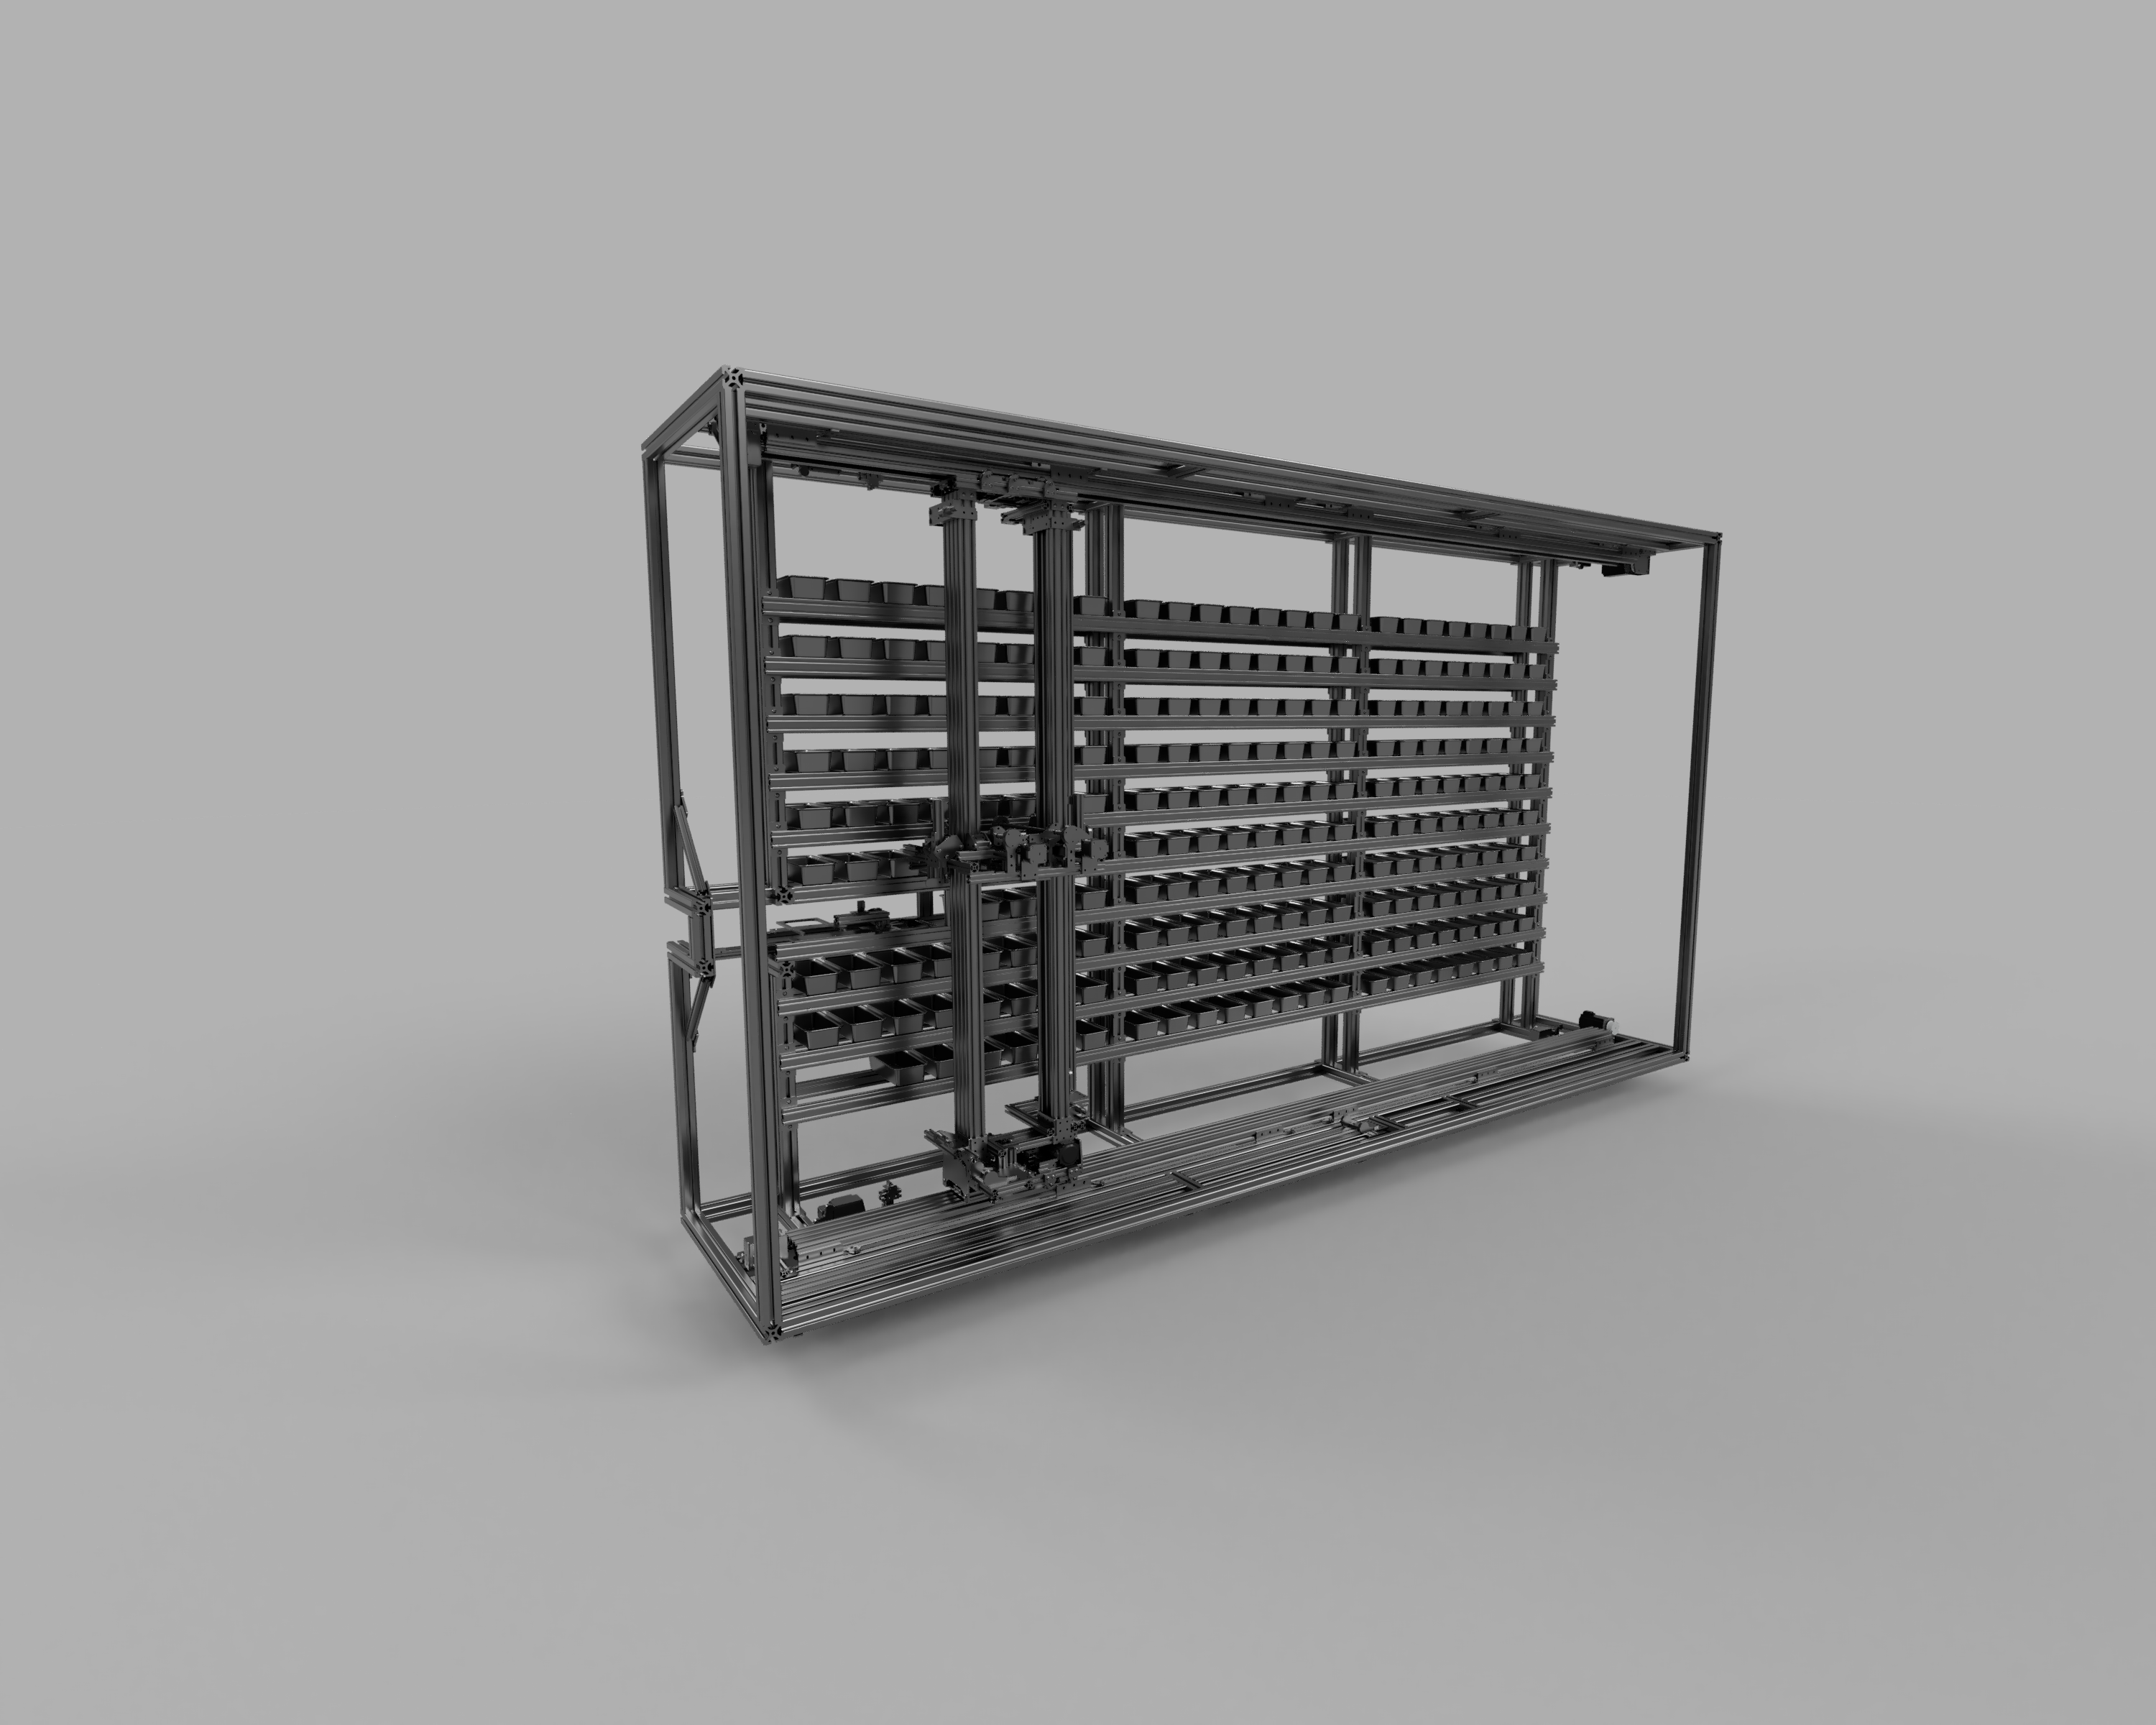
\includegraphics[width=0.3\textwidth]{4f7edc3f-3fba-4cf4-8cb9-5347d889097a.PNG}
    \centering
    \caption{Source may go here: \cite{}}
\end{figure}

\newpage

asd

\printbibliography

\end{document}